% ======================================================================
\chapter{Introduction and background}
\label{ch:background}
% ======================================================================

\section{Motivation}
\label{sec:motivation}

Congestion control (CC) decides how fast a sender may inject data into a shared network. It is one of the oldest control problems in networking: after the Internet's congestion collapses of 1986, Jacobson's slow start and additive-increase/multiplicative-decrease (AIMD) rules restored stability by reacting to packet loss~\cite{jacobson1988congestion,chiu1989analysis}. Almost four decades later the problem takes many forms. Today's flows cross gigabit fiber, shared Wi-Fi, cellular links whose capacity changes every few milliseconds, satellite constellations with frequent handovers, and data-center fabrics where a full round trip takes tens of microseconds. Each environment breaks some assumption of the classic designs. Loss is no longer a reliable congestion signal on wireless links, delay is noisy under ACK aggregation, and buffers range from a few kilobytes in data-center switches to seconds of queueing in cellular base stations. The result is a long line of hand-designed algorithms, each tuned to one environment: Vegas, CUBIC, BBR and Copa for the Internet~\cite{brakmo1995vegas,ha2008cubic,cardwell2016bbr,arun2018copa}, Sprout and Verus for cellular links~\cite{winstein2013sprout,zaki2015verus}, and DCTCP, DCQCN, TIMELY, HPCC and Swift for data centers~\cite{alizadeh2010dctcp,zhu2015dcqcn,mittal2015timely,li2019hpcc,kumar2020swift}.

With reinforcement learning (RL), a controller \emph{learns} its control law instead of having it written by hand. In RL-based congestion control, an agent at the sender (or in the network) watches signals such as delay, throughput, and packet loss. Every short interval it raises or lowers the sending rate or the congestion window, and it receives a reward that is high for fast delivery and low for long delays or lost packets. Over many trials it learns which action works best in each network state. Remy~\cite{winstein2013remy} and PCC~\cite{dong2015pcc,dong2018vivace} showed that machine-generated or online-learned controllers can beat hand-tuned ones. Aurora~\cite{jay2019aurora} then cast Internet congestion control explicitly as a deep RL problem in 2018--2019, and the field has grown quickly since. Our searches retrieved \nIdentifiedTotal{} records, and \nStudies{} primary studies met our eligibility criteria (\cref{sec:method}). However, learned controllers that look excellent in a simulator sometimes fail on links they never saw. Few of them run inside an operating-system kernel, and fewer still have been deployed by an operator.

This survey reviews that literature. It is limited to RL (including imitation learning, offline RL, bandits and multi-agent RL), covers controllers published from 2016 through October 2026, and records for every study \emph{where its results come from}: simulation, emulation, or a real network. That last dimension is our main new contribution. Without it, a reader cannot tell whether a reported gain reflects the network or the simulator.

\section{Research questions and contributions}
\label{sec:rqs}

We organize the survey around three research questions.

\begin{description}[leftmargin=1.2cm,labelwidth=1cm]
  \item[\RQ{1}] \textbf{Design.} How do RL methods control congestion: what do they observe, what do they change, and what reward do they learn from?
  \item[\RQ{2}] \textbf{Testing.} How are these methods trained and tested, and do they still work on networks they did not see in training?
  \item[\RQ{3}] \textbf{Deployment.} What stops operators from using RL-based congestion control in real networks, and what research could fix these problems?
\end{description}

\noindent Our contributions are:
\begin{enumerate}
  \item A systematic, reproducible corpus of \nStudies{} RL/IL congestion-control studies (\nReportsIncluded{} reports), identified with PRISMA~2020~\cite{page2021prisma} from open scholarly indexes, USENIX proceedings, and forward and backward citation searching. Every screening decision and extracted field is released with a reason or an evidence snippet.
  \item A design taxonomy (\RQ{1}) that codes each study's setting, control point, state signals, action, reward terms and RL algorithm family (Chapters~\ref{ch:internet}--\ref{ch:datacenter}).
  \item An evaluation-practice analysis (\RQ{2}, \cref{ch:training}). We code the highest evaluation level reached by every study, the tools used, whether generalization to unseen conditions was tested, and whether code was released. We complement this with a small, fully reproducible case study that shows how the choice of training distribution shapes a learned controller's behavior outside that distribution.
  \item A deployment-barrier analysis and research agenda (\RQ{3}, \cref{ch:deployment}). It maps nine barriers to the studies that address them and reviews the newest work, on congestion controllers designed, tuned or executed by large language models (LLMs).
\end{enumerate}

\paragraph{Roadmap.} The rest of this chapter gives the background needed for the remaining chapters (\cref{sec:cc-primer,sec:rl-primer,sec:formulation}), describes the review method (\cref{sec:method}), positions this survey against earlier ones (\cref{sec:related}), and gives an overview of the corpus (\cref{sec:corpus}). Chapters~\ref{ch:internet}--\ref{ch:datacenter} survey designs by setting: the wide-area Internet; wireless, cellular and satellite networks; and data centers. \Cref{ch:training} covers training and testing, and \cref{ch:deployment} covers deployment barriers, LLM-designed controllers, and open problems.

% ----------------------------------------------------------------------
\section{Congestion control in brief}
\label{sec:cc-primer}

\paragraph{Goals.} A congestion controller should (i) use the available bottleneck capacity (\emph{efficiency}), (ii) avoid standing queues and loss (\emph{low delay}), (iii) share capacity among competing flows (\emph{fairness}, often measured with Jain's index~\cite{jain1984fairness}), (iv) converge quickly and stay stable when conditions change, and (v) coexist with the deployed base, which in practice means not starving CUBIC and BBR flows (\emph{friendliness}). Network utility maximization frames these goals as each flow maximizing a concave utility of its rate~\cite{kelly1998rate}. More recent work argues that deployability should instead be judged by the \emph{harm} a new algorithm inflicts on existing traffic~\cite{ware2019beyond}.

\paragraph{Signals and knobs.} End-to-end controllers infer congestion from what they can measure: packet loss, round-trip time (RTT) and its trend, delivery rate, and Explicit Congestion Notification (ECN) marks set by routers~\cite{rfc3168}. They act through two knobs. The \emph{congestion window} (cwnd) caps the data in flight, so the sending rate is self-clocked by returning ACKs. The \emph{pacing rate} spaces packets in time directly.

\paragraph{Classic end-host algorithms.} \Cref{tab:classic} summarizes the families that RL work compares against. Loss-based AIMD (Reno~\cite{rfc5681}) grows cwnd by one packet per RTT and halves it on loss. Its throughput falls as $1/\sqrt{p}$ with random loss rate $p$~\cite{mathis1997macroscopic}. CUBIC~\cite{ha2008cubic,rfc9438}, the Linux default, grows cwnd as a cubic function of the time since the last loss. Delay-based designs such as Vegas~\cite{brakmo1995vegas} and Copa~\cite{arun2018copa} back off when the RTT rises above its minimum. Model-based BBR~\cite{cardwell2016bbr} estimates the bottleneck bandwidth and minimum RTT and paces at the estimated bandwidth, but its interaction with loss-based flows can be unfair~\cite{ware2019bbr}. Two lines of work anticipate RL directly. Remy~\cite{winstein2013remy} searched offline for a rule table that maximizes an objective under assumed network conditions. A follow-up study showed that such learned controllers degrade when the assumptions are wrong~\cite{sivaraman2014learnability}, the generalization problem this survey revisits. PCC Allegro and Vivace~\cite{dong2015pcc,dong2018vivace} run online micro-experiments at slightly different rates and move toward the rate with higher utility, a function of throughput and loss (and, in Vivace, latency).

\paragraph{Network-assisted control.} Routers and switches influence congestion through active queue management (AQM), which drops or marks packets before the buffer fills: RED~\cite{floyd1993red}, CoDel~\cite{nichols2012codel}, PIE~\cite{rfc8033}, and the L4S architecture with shallow ECN marking~\cite{rfc9330}. In data centers, DCTCP~\cite{alizadeh2010dctcp} reacts to the \emph{fraction} of ECN-marked packets, DCQCN~\cite{zhu2015dcqcn} controls RDMA traffic with ECN-driven rate cuts, TIMELY and Swift~\cite{mittal2015timely,kumar2020swift} use precise delay, and HPCC~\cite{li2019hpcc} uses in-band network telemetry (INT). Their performance depends on parameters that operators tune by hand, most prominently the ECN marking threshold, so several RL studies learn these parameters instead of the end-host control law (\cref{ch:datacenter}).

\begin{table}[t]
\centering
\caption{Classic congestion-control families used as baselines by the RL literature.}
\label{tab:classic}
\small
\begin{tabularx}{\linewidth}{@{}L{2.5cm}L{3.3cm}Y@{}}
\toprule
Family & Examples & Control law (simplified) \\
\midrule
Loss-based AIMD & Reno/NewReno~\cite{rfc5681}, CUBIC~\cite{ha2008cubic} & Grow cwnd until loss; multiplicative decrease on loss. \\
Delay-based & Vegas~\cite{brakmo1995vegas}, Copa~\cite{arun2018copa}, Swift~\cite{kumar2020swift} & Keep queueing delay near a target inferred from RTT minus its minimum. \\
Model-based & BBR~\cite{cardwell2016bbr} & Estimate bottleneck bandwidth and propagation RTT; pace at the estimate and cap in-flight data. \\
Online learning & PCC Allegro/Vivace~\cite{dong2015pcc,dong2018vivace} & Compare a utility of throughput and loss (Vivace: also latency) across rate micro-experiments and move toward the better rate. \\
Offline optimization & Remy~\cite{winstein2013remy} & Search a state-to-action table offline for an objective under an assumed network model. \\
ECN-based (DC) & DCTCP~\cite{alizadeh2010dctcp}, DCQCN~\cite{zhu2015dcqcn} & Switches mark above a queue threshold; senders cut in proportion to the marked fraction. \\
AQM & RED~\cite{floyd1993red}, CoDel~\cite{nichols2012codel}, PIE~\cite{rfc8033} & Router drops or marks early, based on queue length or sojourn time. \\
\bottomrule
\end{tabularx}
\end{table}

% ----------------------------------------------------------------------
\section{Reinforcement learning in brief}
\label{sec:rl-primer}

RL formalizes sequential decision making as a Markov decision process (MDP) $(\mathcal{S},\mathcal{A},P,r,\gamma)$: at each step the agent observes a state $s_t$, takes an action $a_t \sim \pi(\cdot\mid s_t)$, receives a reward $r_t$, and the environment moves to $s_{t+1}$. The goal is a policy that maximizes the expected discounted return $\mathbb{E}\big[\sum_t \gamma^t r_t\big]$~\cite{sutton2018reinforcement}. A congestion controller never sees the whole network, only its own feedback, so the problem is formally a \emph{partially observable} MDP. Most designs compensate by feeding the agent a short history of observations. We group the methods used in the corpus as follows; \cref{fig:rl-families} gives the overall picture.

\begin{itemize}
  \item \textbf{Value-based methods} learn the action-value function $Q(s,a)$. Tabular Q-learning and SARSA suit small discrete state spaces. The Deep Q-Network (DQN)~\cite{mnih2015human} and its variants (double, dueling, Rainbow) approximate $Q$ with a neural network and pick from a discrete set of cwnd or rate adjustments.
  \item \textbf{Policy-gradient methods} optimize $\pi$ directly. Proximal Policy Optimization (PPO)~\cite{schulman2017ppo}, TRPO~\cite{schulman2015trpo} and A3C/A2C~\cite{mnih2016a3c} are the common choices, and they handle continuous rate multipliers naturally.
  \item \textbf{Off-policy actor-critic methods} such as DDPG~\cite{lillicrap2016ddpg}, TD3~\cite{fujimoto2018td3} and SAC~\cite{haarnoja2018sac} reuse past experience from a replay buffer. Distributed variants such as IMPALA~\cite{espeholt2018impala} decouple acting from learning.
  \item \textbf{Offline RL} learns from a fixed dataset of logged interactions without exploring online, e.g., CQL~\cite{kumar2020cql}, CRR~\cite{wang2020crr}, and sequence-modelling approaches such as the Decision Transformer~\cite{chen2021decision}.
  \item \textbf{Imitation learning (IL)} trains a policy to copy an expert, either by behavior cloning or by interactive methods such as DAgger~\cite{ross2011dagger}. In congestion control the expert can be an oracle with full knowledge of a simulated link or an existing heuristic.
  \item \textbf{Bandits and online learning} treat each decision interval as a single-step problem (no state transitions). They are the closest relatives of PCC-style utility ascent.
  \item \textbf{Multi-agent RL (MARL)} trains several interacting agents, for example competing flows or switches, using centralized-training/decentralized-execution methods such as MADDPG~\cite{lowe2017maddpg} and MAPPO~\cite{yu2022mappo}.
\end{itemize}

% ----------------------------------------------------------------------
\section{Congestion control as an RL problem}
\label{sec:formulation}

\Cref{fig:loop} shows the canonical formulation, which Aurora made popular~\cite{jay2019aurora}. Time is divided into \emph{monitor intervals} (MIs). At the start of each MI the agent picks an action, which is applied for the whole interval. When ACKs for that interval return, the sender computes statistics and the reward. Designs vary along five dimensions.

\begin{figure}[t]
\centering
\begin{tikzpicture}[
  node distance=8mm and 14mm,
  box/.style={draw, rounded corners=3pt, align=center, minimum height=10mm, inner sep=5pt, font=\small},
  lab/.style={font=\scriptsize, align=center, text=muted},
  >={Stealth[length=2.2mm]}]
  \node[box, fill=accent!8, minimum width=34mm] (agent) {\textbf{RL agent} $\pi_\theta$\\ (sender, receiver,\\ switch or controller)};
  \node[box, right=26mm of agent, minimum width=30mm] (dp) {\textbf{Datapath}\\ cwnd / pacing rate /\\ ECN threshold};
  \node[box, below=16mm of dp, minimum width=30mm, fill=black!4] (net) {\textbf{Network}\\ bottleneck queue,\\ cross traffic, wireless link};
  \node[box, below=16mm of agent, minimum width=34mm] (stats) {\textbf{Feedback statistics}\\ per monitor interval};
  \draw[->, thick] (agent) -- node[above, lab]{action $a_t$\\(e.g., $x_t = x_{t-1}(1+\alpha a_t)$)} (dp);
  \draw[->, thick] (dp) -- node[right, lab]{packets} (net);
  \draw[->, thick] (net) -- node[below, lab]{ACKs, ECN marks, losses\\(delayed by one RTT)} (stats);
  \draw[->, thick] (stats) -- node[left, lab, xshift=-1mm]{state $s_{t+1}$ (history of $k$ MIs):\\ throughput, RTT, RTT gradient,\\ loss, sending ratio, \dots\\[2pt] reward $r_t = f(\text{thr}, \text{delay}, \text{loss})$} (agent);
\end{tikzpicture}
\caption{The canonical RL congestion-control loop. The agent acts once per monitor interval and observes the consequences one RTT later. Designs differ in where the agent runs, what it observes, what it changes, and how the reward trades throughput against delay and loss.}
\label{fig:loop}
\end{figure}

\begin{enumerate}
  \item \textbf{Placement.} Most agents run at the sender. Some run at the receiver, which is common for real-time video (\cref{sec:rtc}). Network-side agents sit in switches and routers, where they tune ECN or AQM parameters, and a few run in a centralized SDN controller.
  \item \textbf{Observation.} Typical observations are a short history of per-interval statistics: throughput or delivery rate, RTT and its minimum, RTT gradient, loss rate, ECN fraction, the current cwnd or rate, and sometimes cross-layer radio information or in-network telemetry. Aurora deliberately chose \emph{scale-free} features (latency gradient, latency ratio and sending ratio) to help generalization across link speeds~\cite{jay2019aurora}.
  \item \textbf{Action.} The action can set the cwnd or rate directly, usually as a bounded multiplicative change, or tune the parameters of a classic algorithm (an initial window, a BBR pacing gain, a CUBIC parameter). Other designs select among existing algorithms or set network parameters such as ECN thresholds, AQM drop probabilities and buffer sizes. Discrete actions suit value-based methods; continuous actions suit policy-gradient and actor-critic methods.
  \item \textbf{Objective.} Most rewards are weighted combinations of throughput, delay and loss. Aurora, for example, uses $10\cdot\text{throughput} - 1000\cdot\text{latency} - 2000\cdot\text{loss}$ with throughput in packets per second~\cite{jay2019aurora}. Others use Kleinrock's \emph{power} (throughput over delay), PCC-style utility functions, fairness terms, or application-level quality of experience (QoE). The reward fixes the operating point, so it acts as the controller's specification.
  \item \textbf{Decision frequency.} Per-ACK decisions are too expensive for neural inference at line rate. Most designs act once per MI, which ranges from milliseconds to one or more RTTs. Several hybrid designs let a classic algorithm react per ACK while the agent adjusts it at a coarser time scale (\cref{sec:hybrid}).
\end{enumerate}

\noindent Two properties make congestion control harder than the games on which deep RL was popularized. First, the consequences of an action arrive \emph{one RTT later} and are mixed with the effects of other flows' actions, so credit assignment is noisy and the environment is non-stationary. Second, the controller is deployed on networks whose statistics differ from any training environment. Performance under distribution shift therefore says more about a controller than in-distribution reward does (\cref{ch:training}).

% ----------------------------------------------------------------------
% ----------------------------------------------------------------------
\section{Review Method}
\label{sec:method}

We followed the PRISMA~2020 reporting guideline~\cite{page2021prisma}, with the search and snowballing steps adapted to computer science as recommended by Kitchenham and Charters~\cite{kitchenham2007guidelines} and Wohlin~\cite{wohlin2014snowballing}. The whole pipeline (search scripts, raw API responses, every screening decision with its reason, the retrieval log, evidence snippets, and the extraction table) is in the replication package that accompanies this survey (\texttt{review/}). Every number in this section is generated from those files.

\subsection{Eligibility criteria}
\label{sec:eligibility}

\Cref{tab:eligibility} lists the criteria. In short, we include primary studies from 2016--2026 in which a reinforcement-learning or imitation-learning method (including bandits, offline RL and multi-agent RL) controls congestion in a packet network. The method may set a sending rate, a congestion window or pacing rate, the parameters of a congestion-control algorithm, which algorithm runs, or a network-side congestion signal (ECN marking, AQM, buffer sizing). Studies that \emph{evaluate} such controllers (robustness, fairness, verification, interpretability) and frameworks built specifically for training or testing them are included as well, because they bear directly on \RQ{2} and \RQ{3}. Surveys are not primary studies; they are listed separately and discussed in \cref{sec:related}.

Two boundary decisions deserve mention. First, ``congestion control'' in vehicular networks usually means \emph{channel-load} control of periodic safety beacons (decentralized congestion control, DCC). That is a MAC/facilities-layer problem with different objectives, so we exclude it (EC2) and mention it only in \cref{ch:wireless}. Second, adaptive-bitrate video streaming over TCP is excluded (EC2), but rate control for \emph{real-time} media, which replaces WebRTC's Google Congestion Control, is congestion control and is included.

\begin{table}[t]
\centering
\caption{Eligibility criteria.}
\label{tab:eligibility}
\small
\begin{tabularx}{\linewidth}{@{}lY@{}}
\toprule
\multicolumn{2}{@{}l}{\textbf{Inclusion} (all must hold)} \\
IC1 & Packet-switched data network (Internet/WAN, wireless/cellular/satellite, data center, IoT/ad hoc, ICN). \\
IC2 & An RL/IL method (incl.\ bandits, offline RL, MARL) is the controller, or the object of evaluation, and its decision affects how fast sources send or how congestion is signalled. \\
IC3 & Primary study: new controller, evaluation/analysis of RL-based CC, or a training/testing framework built for it. \\
IC4 & Published 2016--2026 in English as a peer-reviewed paper or a preprint with sufficient technical detail. \\
\midrule
\multicolumn{2}{@{}l}{\textbf{Exclusion} (any)} \\
EC1 & ``Congestion'' outside packet networks (road or air traffic, power grids, on-chip interconnects, crowds). \\
EC2 & RL used for another networking task (routing, traffic engineering, load balancing, scheduling, caching, resource allocation, ABR video, MAC/channel access, V2X beacon-load control). \\
EC3 & No RL/IL component (supervised prediction, heuristics, fuzzy logic, metaheuristics, Bayesian optimization). \\
EC4 & Secondary study (survey, review, tutorial, position paper, editorial overview). \\
EC5 & Not a primary research report (thesis or book chapter duplicating published work, proceedings front matter, machine-generated or retracted text, non-English full text). \\
\bottomrule
\end{tabularx}
\end{table}

\subsection{Information sources and search}
\label{sec:search}

The protocol query was
\begin{center}
\small\texttt{("reinforcement learning" OR "imitation learning") AND}\\
\small\texttt{("congestion control" OR "congestion window" OR "ECN")}
\end{center}
applied to titles and abstracts of works published 2016--2026. All searches were run on 31~October~2026. Search strings in each source's syntax are given in \cref{app:search}.

\begin{itemize}
  \item \textbf{OpenAlex} (\nOpenAlex{} records). OpenAlex indexes the records of IEEE Xplore, the ACM Digital Library, Elsevier, Springer, Wiley, MDPI, USENIX and arXiv, and supports Boolean title/abstract search with an open API. We use it as the reproducible stand-in for the subscription databases named in our protocol and attribute each record to its database of origin by DOI prefix: \nOriginIEEE{} IEEE Xplore records (DOI prefix 10.1109) and \nOriginACM{} ACM records (10.1145) among the deduplicated set.
  \item \textbf{arXiv} (\nArxivMatched{} records). The arXiv API's phrase operator under-retrieves (it returned 44 records for the two core phrases against 239 for the same words unquoted). We therefore retrieved on single terms (\nArxivRetrieved{} records) and applied the exact Boolean phrase query locally, treating hyphens as spaces as the subscription databases do.
  \item \textbf{USENIX NSDI and ATC proceedings} (\nUsenixMatched{} records). We scraped the title, authors and abstract of all \nUsenixScanned{} papers in NSDI~2016--2026 and USENIX ATC~2016--2025 (there are no ATC~2026 proceedings) and applied the query locally.
  \item \textbf{Citation searching.} Forward snowballing collected every 2016--2026 work that cites one of ten seed reports of nine landmark studies (Aurora, in its preprint and ICML versions, Orca, Pantheon/Indigo, MVFST-RL, Sage, QTCP, Eagle, TCP-RL and DRL-CC for MPTCP) and mentions ``congestion'' in its title or abstract (\nForwardRetrieved{} works, \nForwardNew{} not already found). Backward snowballing screened the reference lists of sixteen recent included reports with long related-work sections (\nBackwardNew{} new records in range). Finally, \nReviewerKnown{} records known to the reviewers but missed by every search were added and labelled as such.
\end{itemize}

\paragraph{Deviation from the protocol.} Our proposal named IEEE Xplore, the ACM Digital Library and Scopus as sources. Their programmatic search interfaces require institutional API keys, and their web interfaces block scripted queries, so we did not query them directly. OpenAlex covers the same publisher records under an open license and makes the search reproducible by anyone, but it may miss records whose abstracts are absent from its index. Forward and backward citation searching was added to offset this risk. It recovered several well-known studies that the Boolean query cannot match because their abstracts never use the exact phrases: MVFST-RL's abstract, for instance, spells ``ReinforcementLearning'' without a space. The query strings for the three subscription databases are provided in \cref{app:search} so that the search can be repeated with institutional access.

\subsection{Selection process and data collection}
\label{sec:selection}

Records were deduplicated by DOI, arXiv identifier and normalized title (fuzzy similarity above 0.93), and then screened on title and abstract against \cref{tab:eligibility}. Records whose eligibility could not be decided from the abstract went on to full-text assessment. Every decision is stored with a reason code and a one-line justification. For full-text assessment and data collection we retrieved open-access versions (arXiv, author copies, open-access publisher PDFs) for \nFulltext{} of the \nSoughtAll{} reports sought. For the remaining reports, eligibility and data items were assessed from the abstract, the publisher metadata and, where available, a machine-generated summary; data items those sources do not report are coded \emph{not reported} (NR) rather than guessed. Screening and extraction used extensive tool support, namely keyword pre-filtering, automatic mining of candidate evidence (algorithm names, simulator and testbed names, code links, and the sentences that define state, action and reward) and an AI assistant. Every coded value is stored with the source it was coded from (full text, abstract, or reviewers' knowledge), so that it can be audited. \Cref{sec:threats} discusses the resulting limitations. Multiple reports of the same study (for example a conference paper and its journal extension) were linked and counted once as a \emph{study}.

\subsection{Data items}
\label{sec:items}

For each study we coded the items listed in our protocol: the \textbf{setting} (\cref{tab:settings}); the \textbf{control point} (sender, receiver, network device, central controller); the \textbf{RL method} (algorithm and family); the \textbf{state} signals, the \textbf{action} type and the \textbf{reward} terms; the \textbf{training setup}; the \textbf{evaluation environment} at three levels, namely \emph{simulation} (a discrete-event or fluid model, e.g., ns-3, OMNeT++, custom Python simulators), \emph{emulation} (real protocol stacks over emulated links, e.g., Mahimahi, Mininet, NetEm), and \emph{real network} (real links or production traffic, including hardware testbeds); whether \textbf{generalization} to conditions outside the training distribution was explicitly tested; whether \textbf{fairness} or friendliness was evaluated; \textbf{code availability}; and the headline \textbf{result}. Each study's \emph{highest} evaluation level is the most realistic of the three it reports.

\subsection{Study appraisal}
\label{sec:appraisal}

PRISMA asks reviews to assess the risk of bias of included studies. Tools for that purpose, such as those for clinical trials, do not fit engineering studies whose evidence is an experiment the authors designed. We therefore appraise each design study on five \emph{evidence practices} that determine how far its results can be trusted outside the authors' setup. They are: (i) the evaluation environment is reported; (ii) the evaluation includes emulation with real stacks or a real network; (iii) generalization is tested on conditions outside the training range; (iv) fairness or friendliness is evaluated; and (v) code or artifacts are released. The sum is a study's \emph{practice score} from 0 to 5. It appraises the reported evidence, not the merit of the idea, and it is a lower bound for studies coded from abstracts. \Cref{sec:practices} reports the results.

\subsection{Synthesis}
\label{sec:synthesis}

We synthesize narratively by setting (Chapters~\ref{ch:internet}--\ref{ch:datacenter}) and quantitatively across the corpus by tabulating the coded items (\cref{sec:corpus,ch:training}). We do not pool effect sizes. Studies use incomparable baselines, links and metrics, so a meta-analysis of reported gains would be misleading. That incomparability is itself one of our findings.

\paragraph{Registration, funding and competing interests.} The review was not registered. Its protocol is our course project proposal, and \cref{sec:search} reports the deviations from it. The review received no funding, and the authors declare no competing interests. \Cref{app:prisma} maps each PRISMA~2020 item to the place where it is reported.

\begin{figure}[p]
\centering
\begin{tikzpicture}[font=\scriptsize,
  box/.style={draw=black!70, rounded corners=1.5pt, align=left, text width=46mm, inner sep=3pt, fill=white, anchor=north},
  ex/.style={draw=black!70, rounded corners=1.5pt, align=left, text width=44mm, inner sep=3pt, fill=black!3, anchor=north},
  hdr/.style={draw=none, fill=accent!12, align=center, inner sep=3pt, font=\scriptsize\bfseries, anchor=south},
  >={Stealth[length=1.6mm]}]
% columns: databases (x=0), exclusions (x=52mm), other methods (x=105mm); rows: y = 0, -24, -52, -62 mm
\node[box] (id1) at (0,0) {Records identified ($n=567$):\\ OpenAlex: IEEE, ACM, Elsevier, Springer, \dots{} ($n=515$)\\ arXiv API ($n=48$ of 474 retrieved)\\ USENIX NSDI/ATC ($n=4$ of 1,558 papers)};
\node[ex] (dup) at (52mm,0) {Duplicate records removed\\ ($n=63$)};
\node[box] (sc1) at (0,-24mm) {Records screened on title and abstract ($n=504$)};
\node[ex] (ex1) at (52mm,-24mm) {Records excluded ($n=210$):\\ EC1 non-network congestion: 29\\ EC2 other networking task: 112\\ EC3 not RL/IL: 4\\ EC4 secondary study: 34\\ EC5 not a research report: 31};
\node[box] (so1) at (0,-52mm) {Reports sought for retrieval ($n=294$)};
\node[ex] (nr1) at (52mm,-52mm) {Reports not retrieved ($n=11$)};
\node[box] (as1) at (0,-62mm) {Reports assessed for eligibility ($n=283$)};
\node[ex] (ex2) at (52mm,-62mm) {Reports excluded ($n=12$):\\ EC2 ($n=6$), EC3 ($n=1$),\\ EC4 ($n=3$), EC5 ($n=2$)};
\node[box, text width=42mm] (id2) at (105mm,0) {Forward citation search:\\ $n=275$ new (of 446 citing works)\\ Backward citation search:\\ $n=151$ new\\ Known to the reviewers: $n=4$};
\node[box, text width=42mm] (sc2) at (105mm,-24mm) {Records screened ($n=426$)\\ Records excluded ($n=350$)};
\node[box, text width=42mm] (so2) at (105mm,-52mm) {Reports sought ($n=80$)\\ Reports not retrieved ($n=1$)};
\node[box, text width=42mm] (as2) at (105mm,-62mm) {Reports assessed ($n=79$)\\ Reports excluded ($n=19$):\\ EC2 ($n=2$), EC3 ($n=16$), EC4 ($n=1$)};
\node[hdr, text width=46mm] (h1) at ([yshift=2mm]id1.north) {Identification via databases};
\node[hdr, text width=42mm] (h2) at ([yshift=2mm]id2.north) {Identification via other methods};
\node[box, text width=80mm, align=center, fill=accent!6] (inc) at (52mm,-84mm) {\textbf{Studies included in the review: 301}\\ Reports of included studies ($n=331$), including 30 further reports\\ (e.g., journal extensions) of an already included study};
\draw[->] (id1) -- (sc1); \draw[->] (sc1) -- (so1); \draw[->] (so1) -- (as1);
\draw[->] (id1.east |- dup.west) -- (dup.west);
\draw[->] (sc1.east) -- (sc1.east -| ex1.west);
\draw[->] (so1) -- (nr1); \draw[->] (as1.east) -- (as1.east -| ex2.west);
\draw[->] (id2) -- (sc2); \draw[->] (sc2) -- (so2); \draw[->] (so2) -- (as2);
\draw[->] (as1.south) |- ([yshift=4mm]inc.north) -| ([xshift=-12mm]inc.north);
\draw[->] (as2.south) |- ([yshift=4mm]inc.north) -| ([xshift=12mm]inc.north);
\end{tikzpicture}

\caption{PRISMA~2020 flow diagram. Left: identification via databases and registers. Right: identification via other methods (citation searching and records known to the reviewers). ``Reports assessed'' counts full texts where openly available and abstracts plus metadata otherwise (\cref{sec:method}).}
\label{fig:prisma}
\end{figure}

% ----------------------------------------------------------------------
\section{Related surveys and positioning}
\label{sec:related}

Our searches identified \nSecondary{} secondary studies that touch on learning-based congestion control. \Cref{tab:surveys} compares the most relevant of them with this survey, using the scope each one states for itself. Broad surveys of machine learning (ML) or deep RL for networking~\cite{boutaba2018comprehensive,wang2018machine,luong2019applications,tang2021survey} treat congestion control as one application among many. Magazine-style overviews~\cite{zhang2019machine,zhang2020machine,wei2021congestion} discuss a handful of prominent designs and the challenges of standardizing learned controllers. Jiang et al.~\cite{jiang2021when} give the most detailed pre-2021 summary and add an experimental comparison of learning-based schemes. Huang et al.~\cite{huang2021machine} take a broad view of congestion control and avoidance that also covers routing and bandwidth reservation. Later reviews narrow the scope, to wired networks~\cite{lakshmi2022methods}, multipath TCP~\cite{maliha2023survey}, active queue management~\cite{toopchinezhad2025machine}, or fairness~\cite{haque2025fairness}. The two most recent reviews are RL-specific~\cite{li2025survey,abedini2027dynamic}. Abedini et al.\ compare RL algorithms, state/action/reward definitions, simulation platforms and reported outcomes, which is closest to our \RQ{1}. Finally, Vielhaus et al.~\cite{vielhaus2026evaluating} survey \emph{how} congestion-control algorithms in general are evaluated, which complements our \RQ{2}.

This survey differs from them as follows. (i) It is \emph{systematic}: the search, deduplication, screening and extraction are scripted and released with every decision, so the corpus can be audited and updated. (ii) It codes the \emph{evaluation level} (simulation, emulation or real network) of every study, along with generalization testing and code availability, so that claims can be weighed by their evidence. (iii) It covers all settings (Internet, wireless, cellular, satellite, IoT and data centers) through 2026. (iv) It analyzes deployment barriers, including the recent use of LLMs to design controllers, and it adds a reproducible case study on training-distribution shift.

\begin{table}[t]
\centering
\caption{Comparison with prior surveys that cover learning-based congestion control, as described by each survey's stated scope. \cmark: covered; $\circ$: partially or as one topic among many; --: not covered.}
\label{tab:surveys}
\small
\setlength{\tabcolsep}{4pt}
\begin{tabularx}{\linewidth}{@{}L{3.6cm}cYcccc@{}}
\toprule
Survey & Year & Focus & RL-specific & Wireless/DC & Eval.\ level & LLMs \\
\midrule
Luong et al.~\cite{luong2019applications} & 2019 & Deep RL in communications and networking & \cmark & $\circ$ & -- & -- \\
Zhang et al.~\cite{zhang2019machine} & 2019 & ML for Internet CC; standardization challenges & $\circ$ & -- & -- & -- \\
Zhang \& Mao~\cite{zhang2020machine} & 2020 & Selected review of ML for end-to-end CC & $\circ$ & $\circ$ & -- & -- \\
Jiang et al.~\cite{jiang2021when} & 2021 & Learning-based CC survey with experimental comparison & $\circ$ & $\circ$ & $\circ$ & -- \\
Wei et al.~\cite{wei2021congestion} & 2021 & Prominent ML-based CC redesigns compared & $\circ$ & -- & -- & -- \\
Huang et al.~\cite{huang2021machine} & 2021 & ML for broad-sense congestion control and avoidance & $\circ$ & $\circ$ & -- & -- \\
Tang et al.~\cite{tang2021survey} & 2021 & ML for end-to-end communication toward 6G & $\circ$ & $\circ$ & -- & -- \\
Lakshmi \& Arrama~\cite{lakshmi2022methods} & 2022 & RL-based CC in wired networks & \cmark & -- & -- & -- \\
Maliha et al.~\cite{maliha2023survey} & 2023 & MPTCP CC and scheduling, ML vs.\ classic & $\circ$ & $\circ$ & -- & -- \\
Toopchinezhad \& Ahmadi~\cite{toopchinezhad2025machine} & 2025 & ML for active queue management & $\circ$ & $\circ$ & -- & -- \\
Vielhaus et al.~\cite{vielhaus2026evaluating} & 2026 & How CC algorithms are evaluated (not ML-specific) & -- & \cmark & \cmark & -- \\
Li et al.~\cite{li2025survey} & 2025 & Deep RL for CC & \cmark & -- & -- & -- \\
Abedini et al.~\cite{abedini2027dynamic} & 2027 & RL-based CC: algorithms, state/action/reward, platforms & \cmark & $\circ$ & $\circ$ & -- \\
\midrule
\textbf{This survey} & 2026 & Systematic review of RL/IL CC across all settings & \cmark & \cmark & \cmark & \cmark \\
\bottomrule
\end{tabularx}
\end{table}

% ----------------------------------------------------------------------
\section{Overview of the Corpus}
\label{sec:corpus}

The \nStudies{} included studies (\nReportsIncluded{} reports) span 2016 to October~2026. \Cref{tab:all-studies} in \cref{app:tables} lists every study with its setting, action, method, highest evaluation level and code availability. \Cref{fig:trend} shows how quickly the field has grown. Only \nStudiesPreTwentyOne{} studies first appeared before 2021, whereas \nPctSinceTwentyThree{}\% appeared in 2023 or later, with a peak of \nYearMaxN{} studies in \nYearMax{}. The 2026 bar covers ten months only. The Internet/generic group has contributed 20 or more studies every year since 2021 and accounts for most of the growth. IoT and ad hoc studies became noticeably more frequent from 2023, whereas data-center studies remain a small stream of at most six per year.

\begin{figure}[t]
\centering
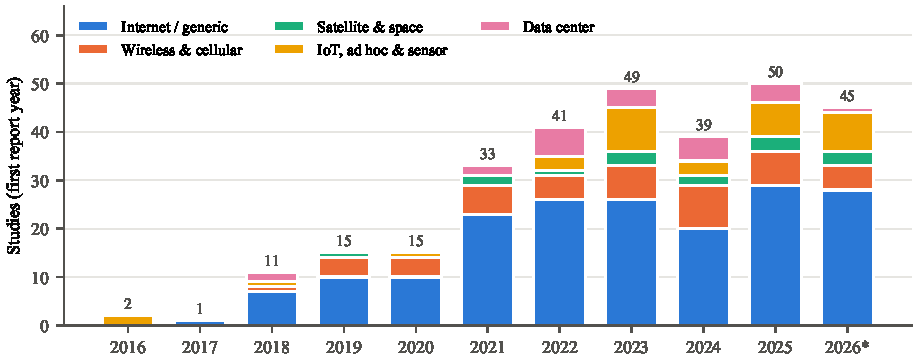
\includegraphics[width=0.86\linewidth]{figures/fig_trend.pdf}
\caption{Included studies by year of first report and setting ($n=\nStudies$). A study with several reports is counted once, in the year of its earliest report. *2026 covers January to October.}
\label{fig:trend}
\end{figure}

\paragraph{Settings.} \Cref{tab:settings} defines the six settings we coded and the chapter that covers each. The largest group consists of studies whose setting is the wide-area Internet (\nSetWan) or a generic wired bottleneck that the authors do not tie to a particular network (\nSetGen). Such ``generic'' studies typically evaluate on a dumbbell topology in ns-3 or Mininet. We discuss both kinds in \cref{ch:internet}, because they share designs, baselines and benchmarks.

\begin{table}[t]
\centering
\caption{Settings coded in this survey, with the number of included studies (all contribution types) and the chapter that synthesizes them.}
\label{tab:settings}
\small
\begin{tabularx}{\linewidth}{@{}lYrl@{}}
\toprule
Setting & What it covers & Studies & Chapter \\
\midrule
Internet / WAN & Paths across the public Internet or a wide-area network; real-time media over the Internet; Pantheon-style evaluations & \nSetWan & \Cref{ch:internet} \\
Generic & A wired bottleneck not tied to a specific network, usually a simulated dumbbell; AQM at a generic router & \nSetGen & \Cref{ch:internet} \\
Wireless \& cellular & Wi-Fi, LTE/5G/mmWave, vehicular and high-speed-rail links, radio fronthaul, multipath over heterogeneous radios & \nSetCell & \Cref{ch:wireless} \\
Satellite \& space & LEO/GEO/HEO satellite links, satellite--ground and space--air--ground integrated networks, deep-space and delay-tolerant links & \nSetSat & \Cref{ch:wireless} \\
IoT, ad hoc \& sensor & Constrained IoT protocols (CoAP, MQTT, 6LoWPAN), wireless sensor networks, MANETs, mesh, smart-grid and industrial IoT & \nSetIot & \Cref{ch:wireless} \\
Data center & Data-center and HPC fabrics, RDMA, ECN tuning at switches, NIC-resident control & \nSetDc & \Cref{ch:datacenter} \\
\bottomrule
\end{tabularx}
\end{table}

\paragraph{Contribution types.} Most studies (\nContribCtrl) propose a new controller. A further \nContribMethod{} contribute a \emph{method} that applies to existing controllers, such as curriculum learning, trace sampling, distillation, reward correction or kernel deployment, and \nContribDeploy{} report a \emph{deployment} in production or an A/B test. The remaining studies do not propose controllers: \nContribAnalysis{} \emph{analyze} existing ones (evaluation, verification, interpretability, attacks) and \nContribFramework{} build \emph{frameworks} for training or testing them. We call the \nDesignN{} studies in the first three groups \emph{design studies}. They are the denominator for the design statistics below.

\paragraph{What the agent changes, and with which algorithm.} \Cref{fig:rl-families} summarizes the coded design items. The two dominant actions are setting the congestion window (\nActCwnd{} studies) and setting the sending or pacing rate (\nActRate). A substantial minority tune the \emph{parameters} of a classic algorithm (\nActParam), select among existing algorithms (\nActSelect), or act inside the network on ECN thresholds, AQM policies or buffer sizes (\nTopicNetSide{} studies across all settings). Algorithm families are coded only when a study names its algorithm, which \nFamKnownN{} of the \nDesignN{} design studies do. Among those, \nPctDeepKnown\% use deep RL, and tabular Q-learning or SARSA account for \nPctTabularKnown\%. Off-policy actor-critic methods (DDPG, TD3, SAC), policy-gradient methods (mostly PPO) and the DQN family are used about equally often. Multi-agent RL (\nFamMarl{} studies) is now common, especially for fairness and in-network control. Imitation, offline and meta-RL remain niche, although several of the most influential designs belong to these families. The agent runs at the sender in \nCtrlSender{} design studies, inside the network in \nCtrlNetwork, at a central (usually SDN) controller in \nCtrlCentral, and at the receiver in \nCtrlReceiver. Receiver-side agents are mostly bandwidth estimators for real-time video; the rest are NDN consumers and individual RDMA and Wi-Fi designs.

\begin{figure}[t]
\centering
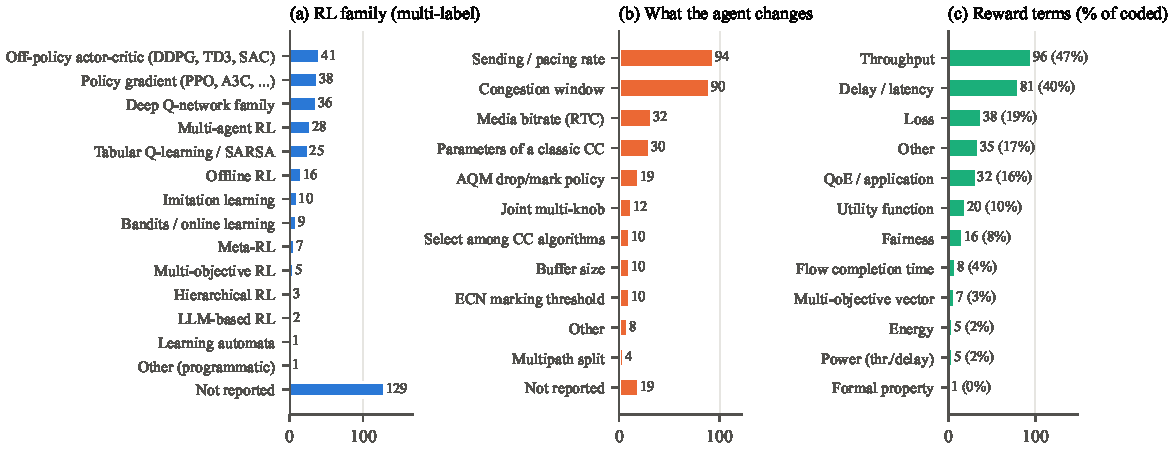
\includegraphics[width=\linewidth]{figures/fig_design.pdf}
\caption{Design items across the \nDesignN{} design studies. (a)~RL family, multi-label: a study combining, e.g., imitation learning and PPO is counted in both. ``Not reported'' means the study does not name its algorithm. (b)~What the agent changes. (c)~Reward terms, as a share of the \nRewardCoded{} studies whose reward is reported.}
\label{fig:rl-families}
\end{figure}

\paragraph{What the agent observes and optimizes.} The state is reported in enough detail to code its signals in \nStateSignalsN{} design studies. Throughput or delivery rate (\nStateThroughputDeliveryRate), delay or RTT (\nStateDelayRtt), loss (\nStateLossDeliveryRatio) and queue occupancy (\nStateQueueBufferInNetwork) dominate. Cross-layer radio information (\nStateCrossLayerRadio), in-network telemetry (\nStateTelemetryNetworkSignals) and ECN marks (\nStateEcnMarks) are rarer. Rewards are reported in \nRewardCoded{} studies. They most often reward throughput (\nRewardThroughput) and penalize delay (\nRewardDelayLatency) and, less often, loss (\nRewardLoss). Others use utility functions, QoE or flow completion time. Only \nRewardFairness{} rewards include an explicit fairness term, which matters for \cref{ch:deployment}.

\paragraph{Hybrid designs.} We call a design \emph{hybrid} when the learned policy works through, alongside, or as a fallback to a classic algorithm rather than replacing it. Examples are an agent that scales CUBIC's window, tunes BBR's gains or a switch's ECN threshold, selects among existing algorithms, or hands over to a heuristic when it is uncertain. Learning \emph{from} classic algorithms only during training, for example by imitating them or by offline RL on their logs, does not make a design hybrid, because the deployed policy then runs alone. Overall, \nPctHybrid\% of design studies are hybrid, rising from \nPctHybridPre\% of those first reported before 2023 to \nPctHybridPost\% since. This is one of the clearest trends in the corpus, and we return to it in \cref{sec:hybrid,ch:deployment}.

\paragraph{Evidence base.} For \nSrcFT{} studies the coding rests on the full text, and for \nSrcKN{} well-known studies whose full text we could not retrieve it rests on the reviewers' knowledge of the paper. The remaining \nSrcAB{} studies were coded from abstracts and metadata. That is why many items are ``not reported'': the abstracts do not say. \Cref{ch:training} therefore reports evaluation practice both for the whole corpus and for the full-text subset, where the coding is complete.

